% Copyright (C) 2012 Shi.Zhan <g.shizhan.g@gmail.com>
%
% Permission is hereby granted, free of charge, to any person obtaining a copy of this software and associated documentation files (the "Software"), to deal in the Software without restriction, including without limitation the rights to use, copy, modify, merge, publish, distribute, sublicense, and/or sell copies of the Software, and to permit persons to whom the Software is furnished to do so, subject to the following conditions:
%
% The above copyright notice and this permission notice shall be included in all copies or substantial portions of the Software.
%
% THE SOFTWARE IS PROVIDED "AS IS", WITHOUT WARRANTY OF ANY KIND, EXPRESS OR IMPLIED, INCLUDING BUT NOT LIMITED TO THE WARRANTIES OF MERCHANTABILITY, FITNESS FOR A PARTICULAR PURPOSE AND NONINFRINGEMENT. IN NO EVENT SHALL THE AUTHORS OR COPYRIGHT HOLDERS BE LIABLE FOR ANY CLAIM, DAMAGES OR OTHER LIABILITY, WHETHER IN AN ACTION OF CONTRACT, TORT OR OTHERWISE, ARISING FROM, OUT OF OR IN CONNECTION WITH THE SOFTWARE OR THE USE OR OTHER DEALINGS IN THE SOFTWARE.
%
% 课程:人机交互技术及应用
% 班级:传播学1001班
% 课时:40学时,2012年秋季1~10周,每周一、三
% 地点:东九楼D212
% 主页:http://code.google.com/p/hci-course/
% 教师:施展 
% 单位:华中科技大学 武汉光电国家实验室
%
\documentclass{beamer}
\usepackage{fontspec,xunicode,xltxtra,beamerthemesplit}
%\usetheme{Hannover} % White background
\usetheme{Berkeley} % Blue background
\setmainfont[
	BoldFont={WenQuanYi Zen Hei},
	ItalicFont={WenQuanYi Micro Hei}
]{WenQuanYi Micro Hei}
\setsansfont[
	BoldFont={WenQuanYi Zen Hei},
	ItalicFont={WenQuanYi Micro Hei}
]{WenQuanYi Micro Hei}

% 中文环境自动换行
\XeTeXlinebreaklocale "zh"
\XeTeXlinebreakskip = 0pt plus 1pt

% 中文环境修正导航栏
\makeatletter
\def\beamer@linkspace#1{
	\begin{pgfpicture}{0pt}{-1.5pt}{#1}{5.5pt}
		\pgfsetfillopacity{0}
		\pgftext[x=0pt,y=-1.5pt]{.}
		\pgftext[x=#1,y=5.5pt]{.}
	\end{pgfpicture}
}
\makeatother

% diagrams
\usepackage{tikz}
\usetikzlibrary{arrows,shapes}

% full page image
\newcommand{\fullPageImage}[2]{
	{
		\usebackgroundtemplate{\includegraphics[width=\paperwidth, height=\paperheight]{#1}}
		\frame[plain]{#2}
	}
}

\title{人机交互技术}
\author{施展}
\institute{华中科技大学~武汉光电国家实验室}
\date{\today}
\titlegraphic{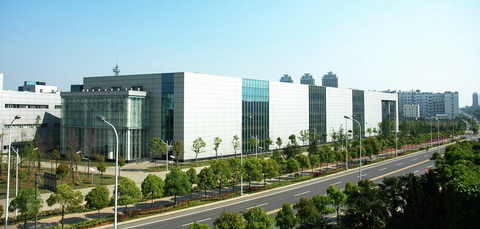
\includegraphics[width=2cm]{images/wnlo.jpg}}

\begin{document}

\begin{frame}
	\titlepage
\end{frame}

\begin{frame}
	\frametitle{内容提要}
	\tableofcontents
\end{frame}

\section{第四讲}
\begin{frame}
	\frametitle{第四讲 交互技术}
	\begin{itemize}
		\item 人机交互输入模式
		\item 基本交互技术
		\item 图形交互技术
		\item 语音交互技术
		%\item 笔交互技术
	\end{itemize}
\end{frame}

\subsection{人机交互输入模式}
\begin{frame}
	\frametitle{人机交互输入模式}
	\beamertemplatetransparentcovereddynamicmedium
	\begin{itemize}[<+->]
		\item 输入设备多种多样;
		\item 对一个应用程序而言,可以有多个输入设备,同一个设备又可能为多个任务服务;
		\item 要求对输入过程的处理要有合理的模式。
		\begin{itemize}
			\item 请求模式 (Request Mode)
			\item 采样模式 (Sample Mode)
			\item 事件模式 (Event Mode)
		\end{itemize}
	\end{itemize}
\end{frame}

\begin{frame}
	\frametitle{人机交互输入模式}
	\beamertemplatetransparentcovereddynamicmedium
	\tikzstyle{block} = [
		rectangle,
		rounded corners,
		draw=black, very thick,
		fill=blue!20,
		text width=8em,
		minimum height=2em,
		text centered]
	\tikzstyle{line} = [
		draw, -latex',
		draw=black, very thick,
		text centered]

	\begin{columns}
		\column{.5\textwidth}
		\begin{itemize}
			\item 请求模式~{\tiny 应用程序驱动设备}
			\begin{itemize}
				\item 在请求模式下,由应用程序负责启动输入设备。
				\item 应用程序执行过程中需要输入数据时,暂停程序的执行,直到从输入设备接受到请求的输入数据后,才继续执行程序。
			\end{itemize}
		\end{itemize}
		\column{.5\textwidth}
		\begin{center}
		\begin{tikzpicture}[node distance=1.5cm, auto,]
			\pause
		    \node [block] (init) {程序工作,输入设备等待程序请求};\pause
		    \node [block, below of=init] (cmd) {收到请求指令};
		    \path [line] (init) -- (cmd);\pause
		    \node [block, below of=cmd] (data) {输入设备工作,程序等待接收数据};
		    \path [line] (cmd) -- (data);\pause
		    \node [block, below of=data] (done) {请求完成}
		    	edge[line, bend right=60] (init.east);
		    \path [line] (data) -- (done);
		\end{tikzpicture}
		\end{center}
	\end{columns}
\end{frame}

\begin{frame}
	\frametitle{人机交互输入模式}
	\beamertemplatetransparentcovereddynamicmedium
	\tikzstyle{block} = [
		rectangle,
		rounded corners,
		draw=black, very thick,
		fill=blue!20,
		text width=6em,
		minimum height=2em,
		text centered]
	\tikzstyle{line} = [
		draw, -latex',
		draw=black, very thick,
		text centered]

	\begin{itemize}
		\item 采样模式~{\tiny 输入设备和应用程序相互独立}
		\begin{itemize}
			% 输入设备连续不断地把信息输入进来,信息的输入和应用程序中的输入命令无关。
			% 应用程序在处理其它数据的同时,输入设备也在工作,新的输入数据替换以前的输入数据。
			% 当应用程序遇到取样命令时,读取当前保存的输入设备数据。
			\item 优点:这种模式对连续的信息流输入比较方便,也可同时处理多个输入设备的输入信息。
			\item 缺点:应用处理滞后,可能丢失信息。
		\end{itemize}
	\end{itemize}
	\begin{center}
	\begin{tikzpicture}[node distance=1.5cm, auto,]
	    \node [] (center) {};\pause
	    \node [block, right of=center] (device) {输入设备工作};\pause
	    \node [block, below of=device] (data) {数据生成}
	    	edge[line, bend right=60] (device.east);
	    \path [line] (device) -- (data);\pause
	    \node [block, below of=center, left of=data] (buffer) {数据缓存区};
	    \path [line] (data) -- (buffer);\pause
	    \node [block, left of=center] (program) {程序工作};\pause
	    \node [block, below of=program] (sample) {数据采样}
	    	edge[line, bend left=60] (program.west);
	    \path [line] (program) -- (sample);
	    \path [line] (buffer) -- (sample);
	\end{tikzpicture}
	\end{center}
\end{frame}

\begin{frame}
	\frametitle{人机交互输入模式}
	\beamertemplatetransparentcovereddynamicmedium
	\tikzstyle{block} = [
		rectangle,
		rounded corners,
		draw=black, very thick,
		fill=blue!20,
		text width=2em,
		minimum height=2em,
		text centered]
	\tikzstyle{queue} = [
		draw, rectangle split,
		rectangle split parts=5, minimum width=1cm, minimum height=0.5cm]
	\tikzstyle{line} = [
		draw, -latex',
		draw=black, very thick,
		text centered]

	\begin{itemize}
		\item 事件模式~{\tiny 输入设备和程序并行工作}
		\begin{itemize}
			\item 输入设备把数据保存到一个输入队列,也称为事件队列,所有的输入数据都保存起来,不会遗失。
			\item 应用程序随时可以检查这个事件队列,处理队列中的事件,或删除队列中的事件。
		\end{itemize}
	\end{itemize}
	\begin{center}
	\begin{tikzpicture}[node distance=1.5cm, auto,]
		\node [] (device) {输入};\pause
		\node [queue, below of=device, right of=device] (R){
			\nodepart{two} \nodepart{three}事件
			\nodepart{four} \nodepart{five}
		};
		\draw [line] (device.east) -| (R.north);\pause
		\node [block, below of=R, right of=R] (poll) {检查};
		\draw [line] (R.south) |- (poll.west);\pause
		\node [block, right of=poll] (handlerA) {{\tiny 事件A处理}};
		\draw [line] (poll.east) -- (handlerA.west);
		\node [block, above of=handlerA] (handlerB) {{\tiny 事件B处理}};
		\draw [line] (poll.east) -- (handlerB.west);
		\node [block, above of=handlerB] (handlerC) {{\tiny 事件C处理}};
		\draw [line] (poll.east) -- (handlerC.west);
	\end{tikzpicture}
	\end{center}
\end{frame}

\begin{frame}
	\frametitle{C10K问题}
	% http://blog.csdn.net/ciaos/article/details/7774209
	\begin{center}
	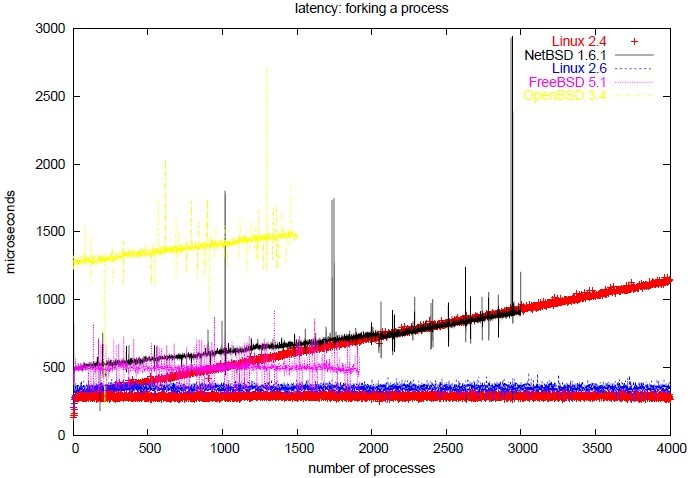
\includegraphics[width=.7\textwidth]{images/c10K.jpg} 
	\end{center}
	\begin{itemize}
	\item 海量用户并发访问显著影响着Web应用服务用户体验
	\end{itemize}
\end{frame}

% http://biancheng.dnbcw.info/python/348697.html
\fullPageImage{images/socket.jpg}{\transwipe}
\fullPageImage{images/epoll.jpg}{\transwipe}
\fullPageImage{images/tornado.jpg}{\transwipe}

\subsection{基本交互技术}
\begin{frame}
	\frametitle{基本交互技术}
	\beamertemplatetransparentcovereddynamicmedium
	\begin{itemize}[<+->]
		\item 定位
		\begin{itemize}
			\item 确定平面或空间的一个点的坐标
			\item 直接定位:用定位设备直接指定某个对象的位置,精确定位。
			\item 间接定位:通过定位设备的运动控制屏幕上的映射光标进行定位,非精确定位。
		\end{itemize}
	\end{itemize}
\end{frame}

% http://wiki.ubuntu.org.cn/Blender2.5x-2.6完全教程_2.1.3
\fullPageImage{images/Blender-tutorial_1.png}{\transwipe}
\fullPageImage{images/Blender-tutorial_2.png}
{
	\transwipe
	\transdissolve<2>
	\pause
	\begin{center}
	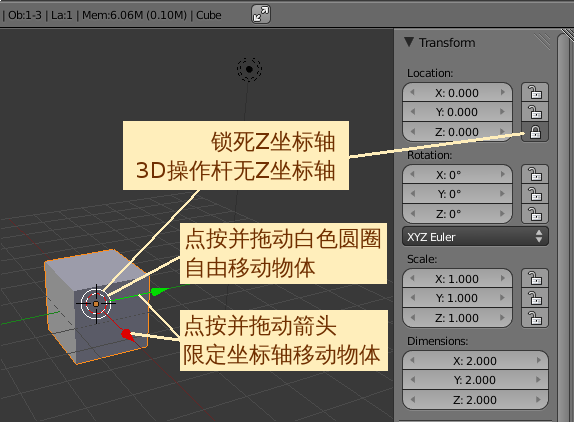
\includegraphics[width=7cm]{images/Blender-tutorial_3.png}
	\end{center}
}

\begin{frame}
	\frametitle{基本交互技术}
	\beamertemplatetransparentcovereddynamicmedium
	\begin{itemize}[<+->]
		\item 笔划
		\begin{itemize}
			\item 输入一组顺序的坐标点
			\item 相当于连续多次调用定位输入
			\item 所输入的点集一般用于显示折线或作为曲线的控制点
		\end{itemize}
	\end{itemize}
\end{frame}

\fullPageImage{images/Blender-tutorial_5.png}{\transwipe}

\begin{frame}
	\frametitle{基本交互技术}
	\beamertemplatetransparentcovereddynamicmedium
	\begin{itemize}[<+->]
		\item 定值
		\begin{itemize}
			\item 定值(或数值)输入用于设置物体旋转角度、缩放比例因子等
		\end{itemize}
	\end{itemize}
\end{frame}

\fullPageImage{images/Blender-tutorial_4.png}{\transwipe}

\begin{frame}
	\frametitle{基本交互技术}
	\beamertemplatetransparentcovereddynamicmedium
	\begin{itemize}[<+->]
		\item 选择
		\begin{itemize}
			\item 在某个选择集中选出一个元素
			\item 通过注视、指点或接触一个对象,使对象成为后续行为的焦点。
		\end{itemize}
	\end{itemize}
\end{frame}

\fullPageImage{images/Blender-tutorial_6.png}{\transwipe}

\begin{frame}
	\frametitle{基本交互技术}
	\transduration{1}<1-3> % Show slide specified number of seconds
	\begin{itemize}
		\item 字符串
	\end{itemize}\pause
	\begin{center}
	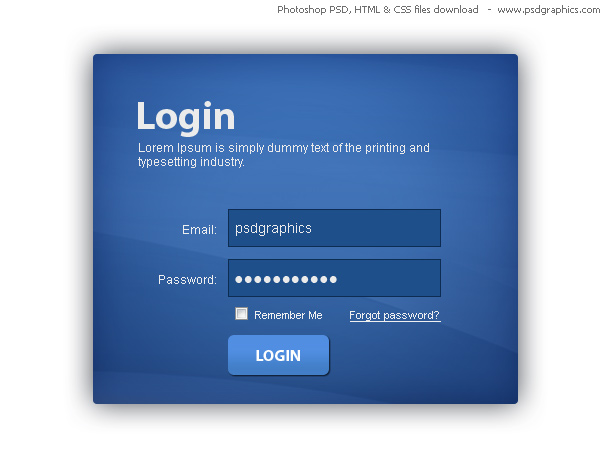
\includegraphics[width=3cm]{images/text-input-1.jpg}~\pause
	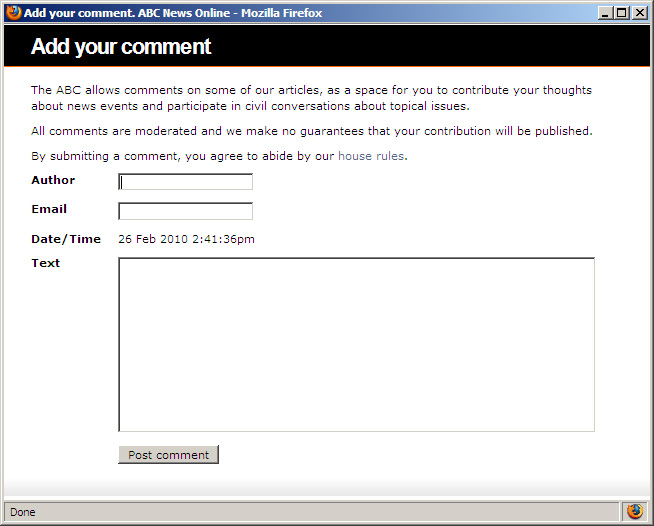
\includegraphics[width=3cm]{images/text-input-2.jpg}~\pause
	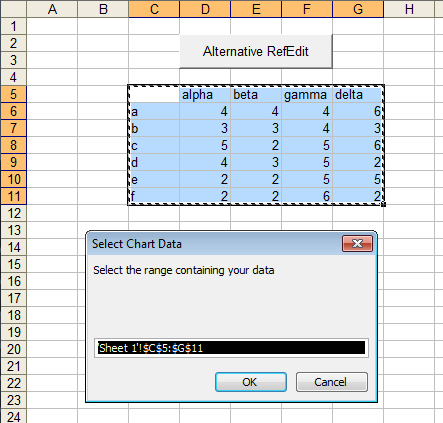
\includegraphics[width=3cm]{images/text-input-3.png}
	\end{center}
\end{frame}

% 身边的例子还有Office软件中Word、PowerPoint里面的图形、表格处理,还有为什么在这里用LaTeX做课件,还可以从图形处理软件的需求出发,引发相关思考,我们需要怎样的图形化输入设备

\subsection{图形交互技术}
\begin{frame}
	\frametitle{图形交互技术}
	\beamertemplatetransparentcovereddynamicmedium
	\begin{itemize}
		\item 技术背景
		\begin{itemize}
			\item WIMP
		\end{itemize}
		\pause
		\item 常用的图形输入技术
		\begin{itemize}
			\item 几何约束
			\item 引力场
			\item 拖动
			\item 橡皮筋
			\item 操作柄
			\item 三维交互
		\end{itemize}
	\end{itemize}\pause
\end{frame}

\begin{frame}
	\frametitle{图形交互技术~{\small WIMP用户界面}}
	\begin{columns}
	\column{.5\textwidth}
	\begin{itemize}
		% http://en.wikipedia.org/wiki/WIMP_%28computing%29
		% http://research.microsoft.com/apps/pubs/default.aspx?id=68165
		\item WIMP界面~\cite{hinckley1996haptic, hinckley2007input}
		\begin{itemize}
			\item 窗口 Windows
			\item 图标 Icons
			\item 菜单 Menus
			\item 指点设备 Pointing Device
		\end{itemize}
		\item 整合上述元素即形成所谓桌面 Desktop
	\end{itemize}
	\column{.5\textwidth}
	% http://en.wikinoticia.com/Technology/general-technology/51006-the-end-of-the-wimp
	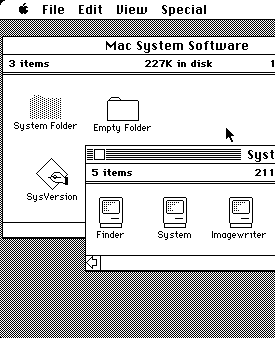
\includegraphics[width=\textwidth]{images/apple-lisa.png}
	\end{columns}
\end{frame}

% http://www.nytimes.com/2009/02/17/science/17map.html?_r=0
% 今后WIMP何去何从?

% http://www.aresluna.org/attached/pics/usability/articles/biurkonaekranie/xerox.big.png
\fullPageImage{images/xerox.big.png}
{
	\transwipe
	\transglitter<2->
	\pause
	\begin{beamerboxesrounded}[shadow=true]{WIMP鼻祖}
	1973年,施乐 Xerox 公司开发了第一款采用 WIMP 概念进行人机交互的操作系统,用于 Xerox Alto 计算机。
	\end{beamerboxesrounded}
	\pause
	\begin{beamerboxesrounded}[shadow=true]{WIMP壮大}
	后继者遍及各个主流平台GUI:\\
	\begin{small}
	Gnome, KDE, Mac OS X, Mac OS, Windows, OS/2,
	BeOS, Amiga, CDE, OpenWindows, NeXTSTEP, GEM, GEOS, RISC OS, Plan 9 \dots
	\end{small}
	\end{beamerboxesrounded}
	\pause
	\begin{beamerboxesrounded}[shadow=true]{WIMP未来}
	\begin{itemize}
		\item WIMP使桌面电脑直观易用
		\item 多任务使桌面电脑过于复杂
		\item 反思人们的需要 \dots
	\end{itemize}
	\end{beamerboxesrounded}
}

\begin{frame}
	\frametitle{图形交互技术~{\small WIMP问题}}
	\beamertemplatetransparentcovereddynamicmedium
	\begin{itemize}[<+->]
		\item 多窗口、多任务的初衷?
		% http://www.forbeschina.com/review/201102/0007520.shtml
		\item 当前的现实情况
		\begin{itemize}
			\item 多任务处理导致工作效率降低
			% 一百万年的进化历程,使得人类大脑一次只能专心处理一项任务。
			% 在追逐猎物或者逃离天敌之时,如果突然将注意力转移到其他事项上,这种行为不会提高我们活下来继续捕猎或者逃生的机会。
	
			% http://health.gmw.cn/2012-07/27/content_4649201.htm
			\item “一心多用”会降低大脑的认知能力
			% 美国《健康》杂志最近载文称,“多管齐下”将会伤害大脑。
			% 美国密歇根大学大脑认知与行为实验室专家表示,多项研究认为,人类大脑总是在不同任务之间不断切换,无法实现多项任务同时完成,大脑其实并不是一个多任务处理器。
			% “一心多用”,不但效率大大降低,而且会降低大脑的认知能力,让你觉得自己变笨了,啥都记不住。
			\begin{itemize}
				\item 多任务操作系统、多标签浏览器、多窗口办公文档编辑、各种网站、各种账户密码、各类提醒
			\end{itemize}		
			% 看一看你的电脑,浏览器开了几个页面,再看看自己的工作状态,发着邮件、听着音乐、间或刷一下微博,有时间再看看淘宝上有什么新货到了,你可能觉得同时处理几个任务效率高。但有的时候,却可能经常会觉得力不从心,比如几个社交网站设了不同的密码,但要到用的时候却怎么都想不起来;手机上设各种备忘录闹钟做提醒;话到嘴边却又忘记说了。
		\end{itemize}		
	\end{itemize}
	\begin{center}
	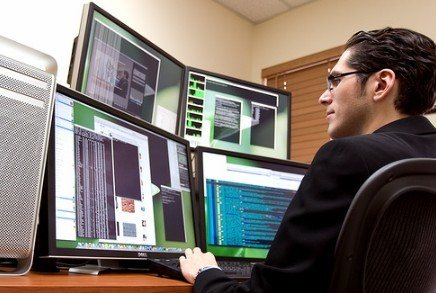
\includegraphics[width=.6\textwidth]{images/multi-task.jpg}
	\end{center}
\end{frame}

\begin{frame}
	\frametitle{图形交互技术~{\small WIMP问题}}
	% http://en.wikinoticia.com/Technology/general-technology/51006-the-end-of-the-wimp
	\beamertemplatetransparentcovereddynamicmedium
	\begin{itemize}[<+->]
		\item 常见任务其实简单:读书、写字、通讯、影音娱乐 % 播放时全屏、读书全屏、挂QQ免打扰 ……
		\item 是否需要多窗口、多任务环境?
		\item 使用习惯上的考虑,除非PC完全由移动+云端所取代!
		\item 对HCI的影响在哪里?
		\begin{itemize}
			\item 手机、平板的窗口、任务管理方法
			\item 界面操作方法
		\end{itemize}
		\item Post-WIMP
		% http://en.wikipedia.org/wiki/Post-WIMP
	\end{itemize}
	\begin{center}
	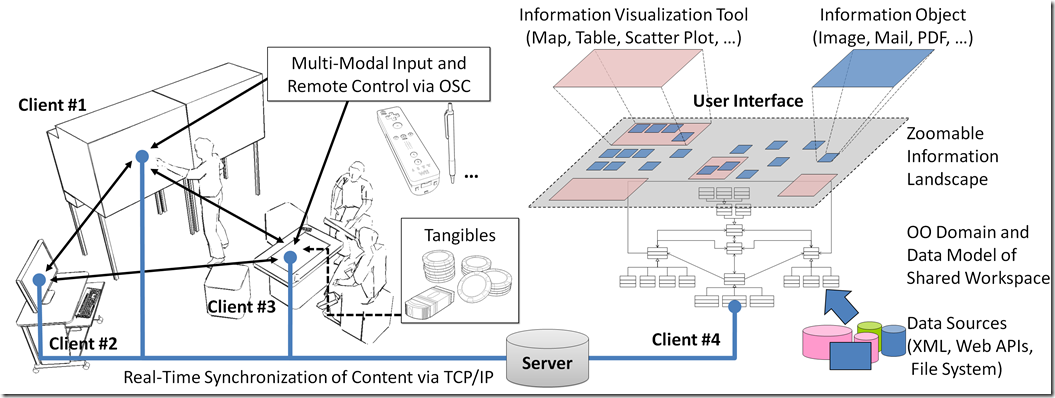
\includegraphics[width=.7\textwidth]{images/post-wimp.png}
	\end{center}
\end{frame}

\begin{frame}
	\frametitle{图形交互技术}
	\begin{itemize}
		\item 几何约束
		\begin{itemize}
			\item 对图形的方向、对齐方式等进行规定和校准
			\item 对定位的约束(网格吸附)
			\item 方向约束
		\end{itemize}
	\end{itemize}
	\begin{center}
	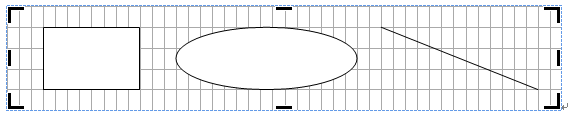
\includegraphics[width=.9\textwidth]{images/grid-word.png}
	\end{center}
\end{frame}

\begin{frame}
	\frametitle{图形交互技术}
	\begin{itemize}
		\item 引力场 Gravity Field
		\begin{itemize}
			\item “吸引到目标图形上”
			\begin{itemize}
				\item 一种定位约束,通过在特定图素(某个目标图形)周围假想有一个区域,当光标中心落在这个区域内时,就自动地被图形上最近的一个点所代替。
			\end{itemize}
			\item 大小要适中
			\item 太小了不易进入引力区,太大了线和线的引力区相交,光标在进入引力区相交部分时可能会被吸引到不希望选的线段上去,增大误接的概率。
		\end{itemize}
	\end{itemize}
	\begin{center}
	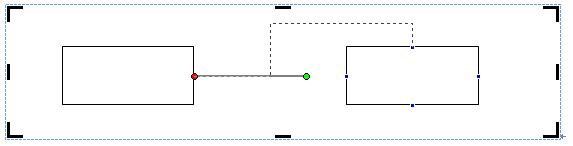
\includegraphics[width=.9\textwidth]{images/gravity-field.png}
	\end{center}
\end{frame}

\begin{frame}
	\frametitle{图形交互技术}
	\begin{itemize}
		\item 橡皮筋 Rubber Band
		\begin{itemize}
			\item 被拖动对象的形状和位置随着光标位置的不同而变化
			\item 不断地进行画图-擦除-画图的过程
		\end{itemize}
	\end{itemize}
	\begin{center}
	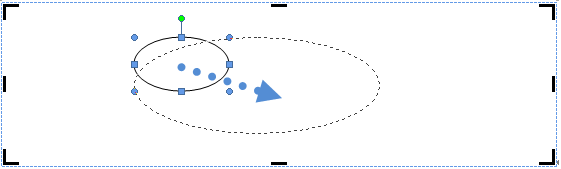
\includegraphics[width=.9\textwidth]{images/rubber-band.png}
	\end{center}
\end{frame}

\begin{frame}
	\frametitle{图形交互技术}
	\begin{itemize}
		\item 操作柄
		\begin{itemize}
			\item 用来对图形对象进行缩放、旋转、错切等几何变换。
			\item 先选择要处理的图形对象,该图形对象的周围会出现操作柄,移动或旋转操作柄就可以实现相应的变换。
		\end{itemize}
	\end{itemize}
	\begin{center}
	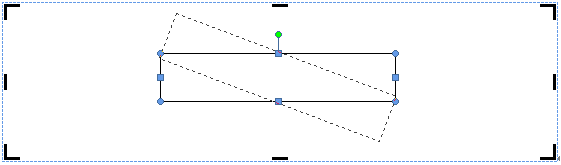
\includegraphics[width=.9\textwidth]{images/handle.png}
	\end{center}
\end{frame}

\begin{frame}
	\frametitle{图形交互技术}
	\begin{itemize}
		\item 拖动 Drag and Drop
		\begin{itemize}
			\item 移动时提供被移动对象的预览显示
			\item 使用户感觉更直观,并可使对象放置的位置更恰当。
			\begin{itemize}
				\item 抽象、简单目标:图像、内容模式
				\item 具体、复杂目标:图形、框线模式
			\end{itemize}
		\end{itemize}
	\end{itemize}
	% http://devheart.org/articles/jquery-customizable-layout-using-drag-and-drop/
	% TODO: jQuery assignment 3 -- Web UI design
	\begin{center}
	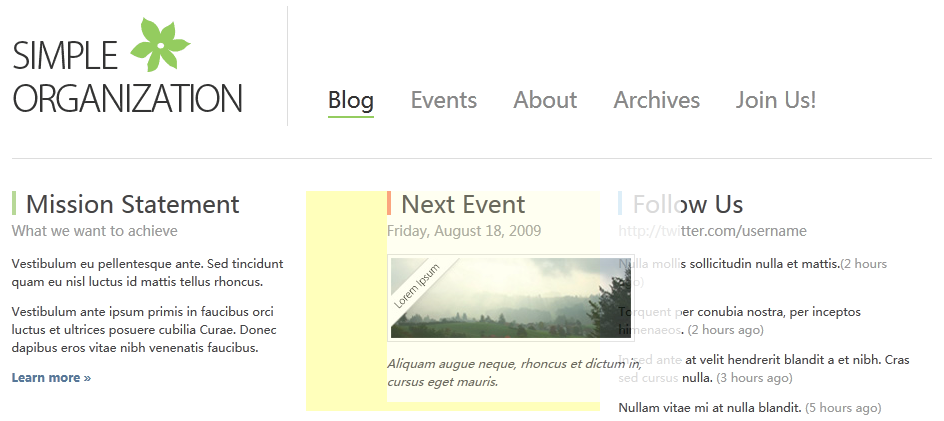
\includegraphics[width=.9\textwidth]{images/drag-and-drop.png}
	\end{center}
\end{frame}

\subsection{语音交互技术}
\begin{frame}
	\frametitle{语音交互技术}
	\beamertemplatetransparentcovereddynamicmedium
	\begin{itemize}
		\item 语音识别
		\begin{itemize}
			\item 让计算机能够把人发出的有意义的话音变成书面语言
		\end{itemize}
		\pause
		\item 语音合成
		\begin{itemize}
			\item 将计算机自己产生的、或外部输入的文字信息转变为可以听得懂的、流利的口语输出
		\end{itemize}
	\end{itemize}
\end{frame}

\begin{frame}
	\frametitle{语音识别}
	\begin{columns}
	\column{.5\textwidth}
	\begin{itemize}
		\item 系统组成
		\begin{itemize}
			\item 语音特征提取
			\item 声学模型与模式匹配
			\item 语言模型与语义理解
		\end{itemize}
		\item 涉及的领域
		\begin{itemize}
			\item 信号处理、模式识别、概率论和信息论、发声机理和听觉机理、人工智能 \dots
		\end{itemize}
	\end{itemize}
	\column{.5\textwidth}
	\only<1>{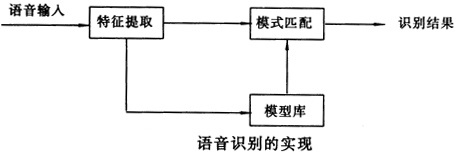
\includegraphics[width=\textwidth]{images/voice-recognition-simple.jpg}}
	% http://www.toshiba.com.cn/aboutus/in_China/yfzx/yjkt/TCH_asr.html
	\only<2>{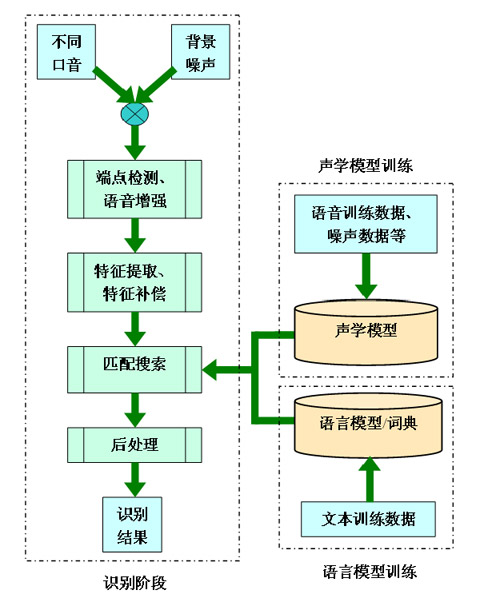
\includegraphics[width=\textwidth]{images/voice-recognition.jpg}}
	\end{columns}
\end{frame}

\begin{frame}
	\frametitle{语音合成}
	\beamertemplatetransparentcovereddynamicmedium
	\begin{itemize}[<+->]
		\item 1939年,贝尔实验室制作出第一个电子语音合成器VODER,是一种利用共振峰原理所制作的合成器。
		\item 1960年,瑞典语言学家G. Fant则提出利用线性预测编码技术(LPC)来作为语音合成分析技术,并推动了日后的发展。
		\item 1980年代,Moulines E和Charpentier F提出新的语音合成算法PSOLA,此技术可以合成比较自然的语音。
	\end{itemize}
\end{frame}

\begin{frame}
	\frametitle{语音合成}
	\beamertemplatetransparentcovereddynamicmedium
	\begin{itemize}
		\item TTS的基本结构
		\pause
		\begin{itemize}
			\item 语言学处理
			\begin{itemize}
				\item 模拟人对自然语言的理解过程——文本规整、词的切分、语法分析和语义分析,使计算机对输入的文本能完全理解,并给出后两部分所需要的各种发音提示。
			\end{itemize}
			\pause
			\item 韵律处理
			\begin{itemize}
				\item 为合成语音规划出音段特征,如音高、音长和音强等,使合成语音能正确表达语意,听起来更加自然。
			\end{itemize}
			\pause
			\item 声学处理
			\begin{itemize}
				\item 根据前两部分处理结果的要求输出语音,即合成语音。
			\end{itemize}
		\end{itemize}
		\pause
		\item 在语音合成技术的发展过程中
		\begin{itemize}
			\item 早期的研究主要是采用参数合成方法,后来随着计算机技术的发展又出现了波形拼接的合成方法。
		\end{itemize}
		\pause
		\item 现在主要有
		\begin{itemize}
			\item 共振峰合成、LPC合成、PSOLA拼接合成和LMA声道模型技术 \dots
		\end{itemize}
	\end{itemize}
\end{frame}

\begin{frame}
	\frametitle{语音合成~{\small 应用实践}}
	\beamertemplatetransparentcovereddynamicmedium
	\begin{itemize}
		\item Speech SDK/SAPI
		\begin{itemize}
			\item Microsoft Speech SDK 5.1 \textbf{\url{http://www.microsoft.com/en-us/download/details.aspx?id=10121}}
		\end{itemize}
		\pause
		\item eSpeak
		\begin{itemize}
			\item A compact open source software speech synthesizer \textbf{\url{http://espeak.sourceforge.net/}}
		\end{itemize}
		\pause
		\item Speech API Community Group
		\begin{itemize}
			\item Produce a JavaScript Speech API \textbf{\url{http://www.w3.org/community/speech-api/}}
			\item 2012-06-13 Speech JavaScript API \textbf{\url{http://dvcs.w3.org/hg/speech-api/raw-file/tip/speechapi.html}}
		\end{itemize}
	\end{itemize}
\end{frame}

\fullPageImage{images/linux-espeak.jpg}{\transwipe}

%\subsection{笔交互技术}
%\begin{frame}
%	\frametitle{笔交互技术}
%
%\end{frame}

\section{小结}
\begin{frame}
	\frametitle{小结}
	\begin{itemize}
		\item 理解人机交互输入模式
		\item 了解主要交互技术
	\end{itemize}
\end{frame}
 
\begin{frame}
	\frametitle{参考文献}
	\bibliographystyle{plain}
	\bibliography{hci}
\end{frame}

\end{document}